\subsection{The Disordered Ising Model}
\label{ssec:isingmodel}
    The examined model is a 2D Ising model.
    The most common definition of the Ising model, to which will be referred to
    as the \emph{square lattice Ising model}, is a square lattice with
    edge length \(L\) and \(N=L^2\) sites with periodic boundary conditions.
    Note that \(N\) always refers to the number of sites in this thesis.
    Each site has a magnetic moment, which is called the spin. Each
    spin can take a value \(s \in \{-1,+1\}\) and interacts with its
    nearest neighbors described by the Hamiltonian
    \begin{equation}
        H = - \sum_{\avg{i,j}}J_{ij}s_{i}s_{j}.
        \label{eq:hamiltonian}
    \end{equation}
    \(\avg{i,j}\) refers to nodes \(i\) and \(j\) which are nearest
    neighbors, so that they are directly coupled to each other. The
    coupling between \(i\) and \(j\) is characterized by \(J_{ij}\),
    the coupling constant. If \(J_{ij} > 0 \ \forall \avg{i,j}\) the model resembles a ferromagnet.
    For the square lattice Ising model \(J_{ij} = 1 \ \forall \avg{i,j}\) applies.\\
    The most important modification of the square lattice Ising model in this
    thesis is that the sites of the square lattice are displaced introducing
    geometric disorder resulting in a non regular graph structure.
    The displacement is randomly Gaussian distributed with standard
    deviation \(\sigma\), i.e.\ the \(x\) and \(y\) coordinates of the
    sites are displaced by random \(\Delta x\) and \(\Delta y\) drawn
    from a Gaussian distribution
    \begin{equation}
        f(x)=\frac{1}{\sqrt{2\pi}\sigma}\mathrm{e}^{-\frac{x^2}{2\sigma^2}}.
        \label{eq:gauss}
    \end{equation}
    This is sketched in Fig.\ \ref{fig:displacement}.
    \begin{figure}[htbp]
        \centering
        \begin{tikzpicture}[scale=1.5, declare function={
        normal(\x,\m,\y) = 1/exp((\x-\m)*(\x-\m)/2/(\s^2))-\y;
      }]
    \def\s{0.5}

    \draw[dashed] (-2,0) -- (4,0);
    \draw[dashed] (0,-2) -- (0,2);
    \draw[dashed] (2,-2) -- (2,2);

    \def\dxa{0.4}
    \def\dya{-0.8}

    \draw (\dxa,\dya) -- node [below] {$\Delta x$} (0,\dya);
    \draw (\dxa,\dya) -- node [right] {$\Delta y$} (\dxa,0);
    \draw[loosely dotted] (\dxa,0) -- (\dxa,{1.6+normal(\dxa,0,0)});
    \draw[loosely dotted] (0,\dya) -- ({-1.6-normal(\dya,0,0)},\dya);
    \draw[->] (0,0) -- (0+\dxa*0.9,0+\dya*0.9);

    \draw[color=black,domain=-1.5:1.5] plot [smooth] (\x,{normal(\x,0,0)+1.6}) node[right] {};
    \fill (0, 0) circle(0.08);
    \draw[color=black] (0+\dxa, 0+\dya) circle(0.08);
    \draw[color=black,domain=-1.5:1.5,rotate=90] plot [smooth] (\x,{normal(\x,0,0)+1.6}) node[right] {};

    \draw[|-|] (-\s,2.8) -- node [above] {$\sigma$} (\s,2.8);
    \draw[|-|] (-2.8,-\s) -- node [left] {$\sigma$} (-2.8,\s);


    \def\dxb{0.5}
    \def\dyb{0.2}

    \draw[color=gray] (2+\dxb,0+\dyb) -- node [above] {$\Delta x_{2}$} (2, \dyb);
    \draw[color=gray] (2+\dxb,0+\dyb) -- node [right] {$\Delta y_{2}$} (2+\dxb,0);
    \fill[color=gray] (2, 0) circle(0.08);
    \draw[color=gray] (2+\dxb, 0+\dyb) circle(0.08);
\end{tikzpicture}

        \caption[Sketch how the Displacement works]
        {
            Sketch how the displacement of the nodes works. The nodes
            get displaced by \(\Delta x\) and \(\Delta y\) drawn from the
            distributions displayed next to the points. The original
            square lattice is indicated by dashed lines.
        }
        \label{fig:displacement}
    \end{figure}\\
    In the following \(\sigma\) will also be called \emph{disorder parameter}.
    If we take "nearest neighbor" in the Euclidean meaning, most sites
    will only have one nearest neighbor after the
    displacement. If only the edges between these neighbors remained,
    the lattice would collapse to many very small clusters. But if one
    left the edges as the were before the displacement, the edges would
    cross -- at least for big displacements. The crossing of edges then
    would destroy the planar character of the model.
    To avoid this, a new edge set will be etablished after the displacement.
    The edges are constructed according to
    one of the two in Sec.\ \ref{ssec:graphtypes} defined rules,
    so that for a given configuration of points the resulting graph is an
    instance of a proximity graph. The coupling constant \(J\) gets
    identified with edge weights. \(J\) will be changed to depend on the
    geometric distance between the connected pair of sites. More precise,
    the weight of an edge is \(E_{ij} = J_{ij} = \exp (\alpha (1-d_{ij}))\)
    where \(d_{ij}\) is the Euclidean
    distance between the nodes \(i\) and \(j\). Following Ref.\ \cite{Lima2000}
    the free parameter \(\alpha\) is set to \(\alpha = 0.5\).
    The boundary is periodic, i.e.\ nodes near the right edge can be
    connected to nodes near the left edge and vice versa. Analogously the
    top and bottom edges are connected. One can imagine that the model
    lives on the surface of a torus as pictured in Fig.\ \ref{fig:torusRNG}.
    In subsequent graphics the graphs will be unwrapped to rectangular
    shapes. Connections which cross a periodic boundary are indicated
    by edges which connect a solid node to a dashed node.
    \begin{figure}[htbp]
        \centering
        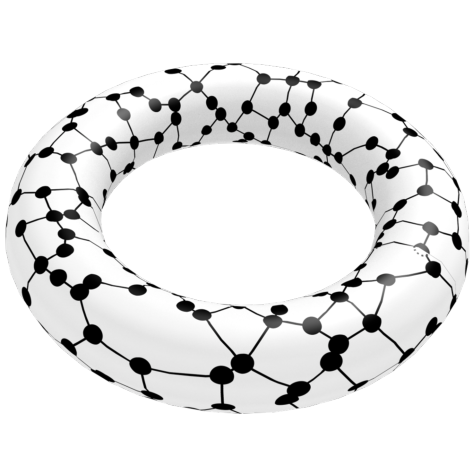
\includegraphics[width=0.45\textwidth]{images/torus}
        \caption[A Graph on a Torus to Visualise Periodic Boundary Conditions]
        {
            A graph on a torus to visualize periodic boundary conditions.
            On this torus, for a more clear presentation, the underlying
            graph exhibits a height to width ratio of 1:4. At 1:1 the torus would cut
            itself. Hence, the torus represents the geometry of the model
            not perfectly, but gives very quick the right idea.
            Also the shades are of course only a guide to the eye.
        }
        \label{fig:torusRNG}
    \end{figure}\\
    Note that for \(\sigma = 0\) all \(d_{ij} = 1\) and therefore all
    \(J_{ij} = 1\), so that the disordered Ising model is reduced to the
    square lattice Ising model. For this an analytic solution exists \cite{Onsager1944}.
    The critical temperature is
    \begin{equation}
        T_c = 2J/\ln(1+\sqrt 2) = 2.2691...
        \label{eq:exactTc}
    \end{equation}
    and the critical exponents are \(\alpha = 0\), \(\beta = \frac{1}{8}\)
    and \(\gamma = \frac{7}{4}\). These values are universal for the Ising
    model. Their meaning will be explained in Sec.\ \ref{ssec:critExp} in more detail.\\
    The case for randomly distributed sites \(\sigma \gtrsim 1\) is
    already studied on a Delaunay triangulation. Ref.\ \cite{Janke1994} examines
    this for constant \(J\) and Ref.\ \cite{Lima2000} for
    \begin{equation}
        J_{ij} = e^{-\alpha d_{ij}}.
        \label{eq:coupling}
    \end{equation}
    Both articles conclude that this model lies within the universality
    class of the square lattice Ising model, i.e.\ has the same critical
    exponents, as can be expected since the underlying graph structure can
    be embedded in 2D. Hence, due to universality it should exhibit the same
    critical exponents as the basic square lattice Ising ferromagnet.

\subsection{Proximity Graphs}
\label{ssec:graphtypes}
    A graph \(G(V,E)\) is a set of nodes \(V\) and edges \(E\). In the
    scope of this model, the nodes get identified with the sites of the
    lattice and the edges signal the neighbor status of two sites. If the
    corresponding nodes are connected, the sites will be neighbors.\\
    All here mentioned graph types are \emph{proximity graphs}.
    The edges of these graphs connect nodes which are by some metric near
    to each other.
    Hence they are suited to generalize problems defined on regular
    lattices with nearest neighbor relationships.
    In this thesis the distance is always determined by the Euclidean
    metric in two dimensions, though in principle every metric in any
    dimension can be used.\\

    \subsubsection{Delaunay Triangulation}
        The Delaunay triangulation (DT) is an undirected graph. An edge
        between two nodes \(i\) and \(j\) will be drawn, if there exists
        a circle passing through \(i\) and \(j\), which does not contain
        any other node in its interior, see Ref.\ \cite{Katajainen}.
        To make this clear a the construction of a four node DT is sketched
        in Fig.\ \ref{fig:def:DT} in the appendix Sec. \ref{appendix:DT_def}.

    \subsubsection{Gabriel Graph}
        The Gabriel graph (GG) \cite{Gabriel1969}
        is a subgraph of the DT, i.e.\ for the same set of nodes
        \(V\) the edge set of the DT is a superset of the edge set of the
        GG \(E_{DT} \supseteq E_{GG}\). Two nodes \(i\) and \(j\) with distance
        \(d_{ij}\) will be connected with an edge, if a circle with its
        center on half way between \(i\) and \(j\) and radius
        \(r = \frac d 2\) contains no other nodes. This area will be
        called \emph{lune} in the following. See also the cross hatched region
        from Fig.\ \ref{fig:lunes}\subref{sfig:lunes:def}.

    \subsubsection{Relative Neighborhood Graph}
        The Relative Neighborhood
        graph (RNG) \cite{Toussaint1980} is a subgraph of the GG. Two nodes \(i\) and \(j\) with
        distance \(d_{ij}\) will be connected, if no other node is in the
        \emph{lune}. The lune is defined as the intersection of two
        circles with radius \(r = d\) and centers on \(i\) and \(j\).
        See also the hatched region in Fig.\ \ref{fig:lunes}\subref{sfig:lunes:def}.

    \begin{figure}[htbp]
        \centering
        \subfigure[Definition of the Lunes][]{
            \label{sfig:lunes:def}
            \tikzset{
    hatch distance/.store in=\hatchdistance,
    hatch distance=10pt,
    hatch thickness/.store in=\hatchthickness,
    hatch thickness=2pt
}

\makeatletter
\pgfdeclarepatternformonly[\hatchdistance,\hatchthickness]{flexible hatch no}
{\pgfqpoint{0pt}{0pt}}
{\pgfqpoint{\hatchdistance}{\hatchdistance}}
{\pgfpoint{\hatchdistance-1pt}{\hatchdistance-1pt}}%
{
    \pgfsetcolor{\tikz@pattern@color}
    \pgfsetlinewidth{\hatchthickness}
    \pgfpathmoveto{\pgfqpoint{0pt}{0pt}}
    \pgfpathlineto{\pgfqpoint{\hatchdistance}{\hatchdistance}}
    \pgfusepath{stroke}
}
\makeatletter
\pgfdeclarepatternformonly[\hatchdistance,\hatchthickness]{flexible hatch nw}
{\pgfqpoint{0pt}{0pt}}
{\pgfqpoint{\hatchdistance}{\hatchdistance}}
{\pgfpoint{\hatchdistance-1pt}{\hatchdistance-1pt}}%
{
    \pgfsetcolor{\tikz@pattern@color}
    \pgfsetlinewidth{\hatchthickness}
    \pgfpathmoveto{\pgfqpoint{0pt}{\hatchdistance}}
    \pgfpathlineto{\pgfqpoint{\hatchdistance}{0pt}}
    \pgfusepath{stroke}
}

\begin{tikzpicture}
    \clip (-2,2.25) rectangle (2,-1.75);

    \begin{scope}
        \clip (-1, 0.5) circle(2.06155281281);
        %~ \fill[fill=blue!20] (1, 0) circle(2.06155281281);
        %~ \draw[pattern=north west lines] (1, 0) circle(2.06155281281);
        \draw[pattern=flexible hatch no,hatch distance=10pt,hatch thickness=0.7pt] (1, 0) circle(2.06155281281);
    \end{scope}

    %~ \fill[fill=white] (0, 0.25) circle(1.0307764064);
    %~ \draw[pattern=north east lines] (0, 0.25) circle(1.0307764064);
    \draw[pattern=flexible hatch nw,hatch distance=10pt,hatch thickness=0.7pt] (0, 0.25) circle(1.0307764064);
    \draw[thick] (0, 0.25) circle(1.0307764064);

    \draw[thick] (-1, 0.5) circle(2.06155281281);
    \fill (-1, 0.5) circle(0.1);
    \draw[thick] (1, 0) circle(2.06155281281);
    \fill (1, 0) circle(0.1);
    \draw[thick] (1, 0) -- (-1, 0.5);
\end{tikzpicture}

        }
        \subfigure[RNG example][]{
            \label{sfig:lunes:rng}
            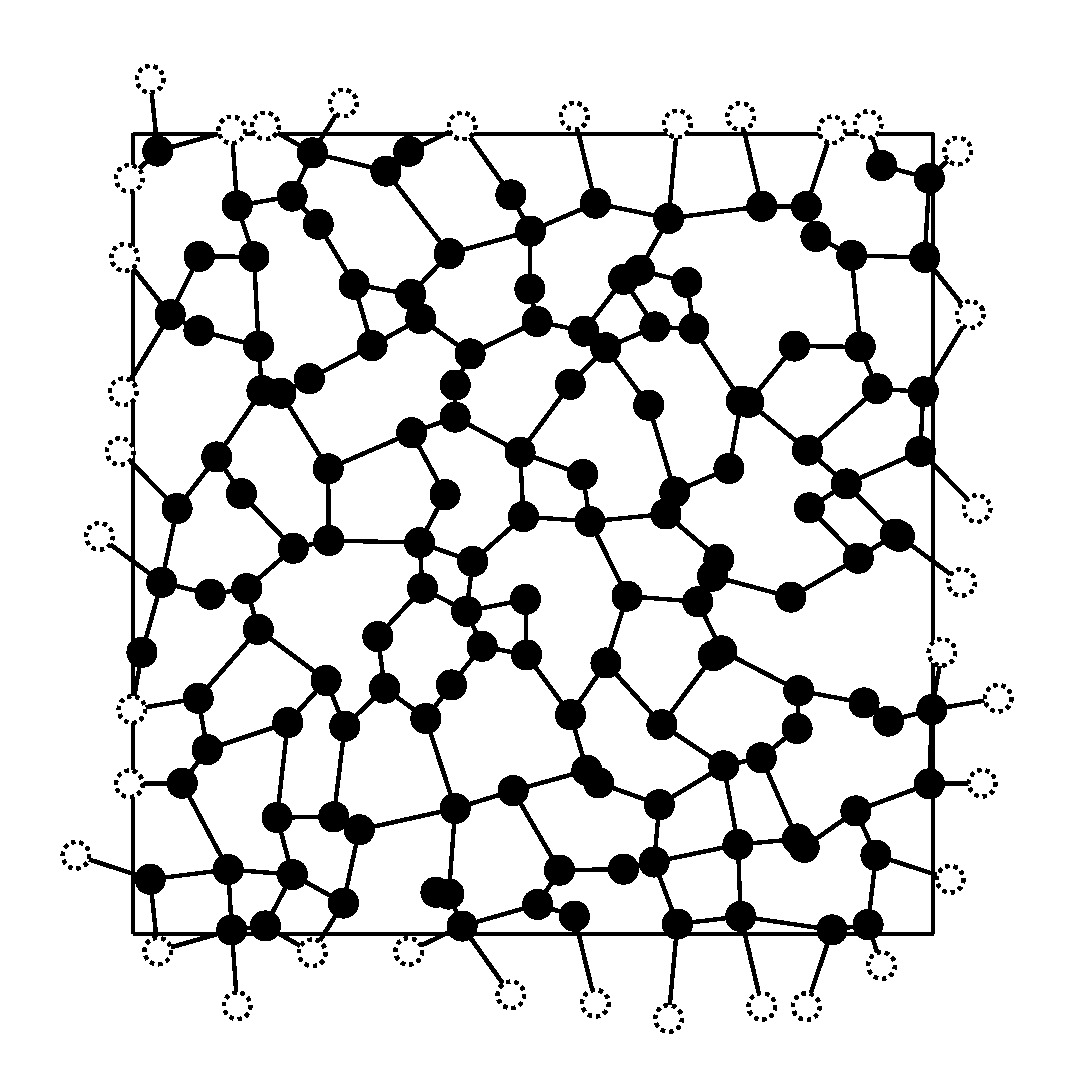
\includegraphics[width=0.3\textwidth]{images/RNG/L12S03.pdf}
        }
        \subfigure[GG example][]{
            \label{sfig:lunes:gg}
            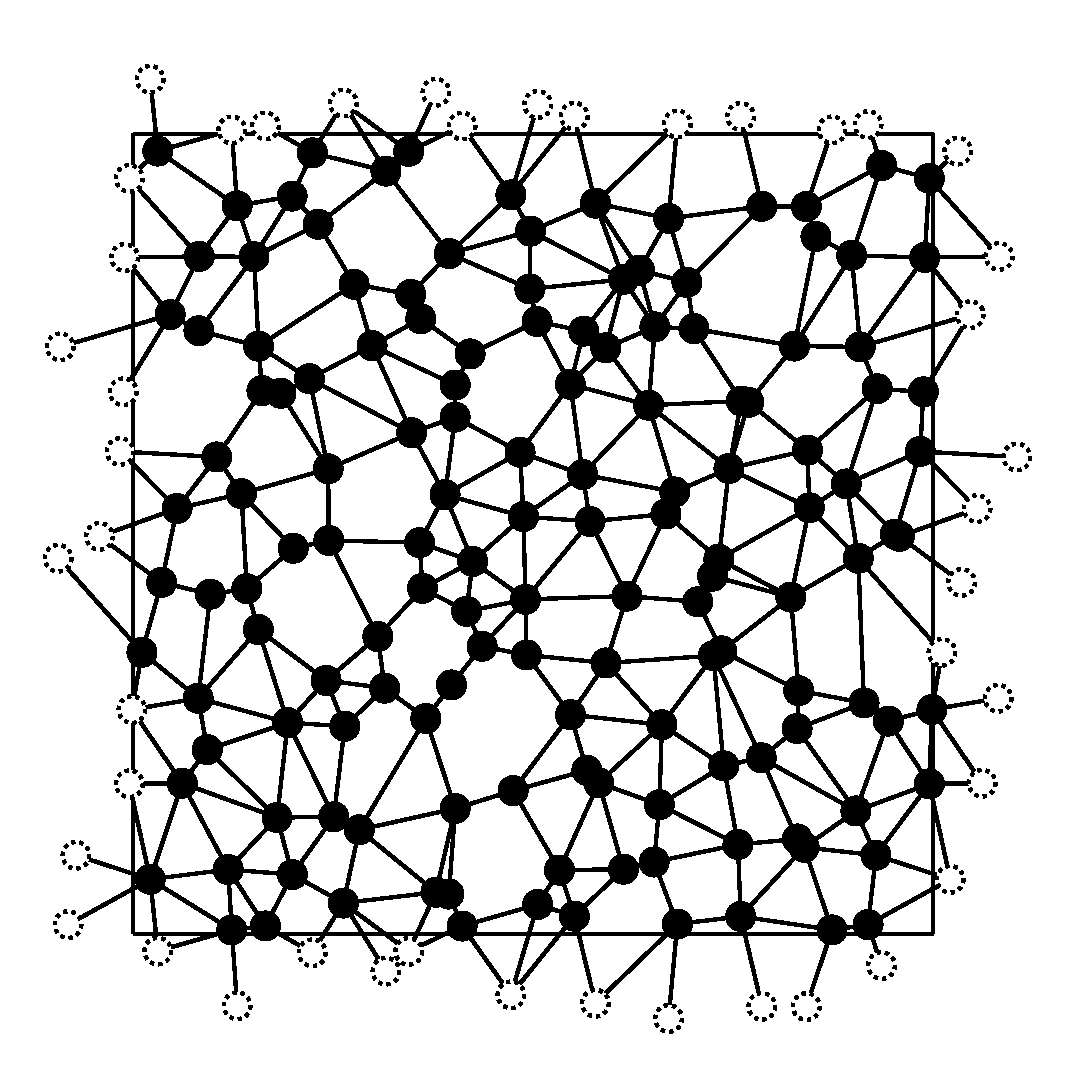
\includegraphics[width=0.3\textwidth]{images/GG/L12S03.pdf}
        }
        \caption[Gabriel - and Relative Neighborhood Graph]
        {
            \subref{sfig:lunes:def} Lunes, which define where an edge
                exist, of RNG (hatched region) and GG (cross hatched region).
                It is evident from this sketch that the GG is a supergraph
                of the RNG. If there is an edge in the RNG, the hatched
                region contains no node, the of course also the double
                hatched region contains no node and thus this edge appears
                also in the GG. So every egde of the RNG is also present
                in a GG on the same node set.
            \subref{sfig:lunes:rng} Example of a RNG on periodic
                boundary conditions. Periodic nodes are dashed.
            \subref{sfig:lunes:gg} Example of a GG on
                periodic boundary conditions. Periodic nodes are dashed.
        }
        \label{fig:lunes}
    \end{figure}

    \subsubsection{Construction}
        The simplest way to construct these graphs is to test for each
        pair of nodes if any other node lies in
        the lune of the pair. That is of complexity \(O (N^3)\), because
        there are \(N(N-1)\) pairs and for each \((N-2)\) nodes to test. So
        the running time of a straight forward implementation would be of
        order \(O(N^3)\).\\
        To reduce the complexity one can first create a DT in complexity \(O (N \log N)\)
        \cite{RNGCell} and test the connectedness for each edge contained
        therein, because the DT is a supergraph of both.
        For the construction of the DT for a given set of points one might
        use existing software libraries, e.g.\ the \texttt{qHull}\footnote{\url{http://www.qhull.org}} library.
        However, generation of the graphs is not time critical in the scope
        of this bachelor thesis.\\
        So a trade off is to use basically the simple method but only test
        the connectedness for nodes which are near to the lune and abort if
        one node inside the lune is found. To determine which nodes are
        near the lune one can subdivide the area in \(M\) \emph{cells} of size
        \(L_c \times L_c\) and save for each cell a list with nodes lying
        inside like presented in Ref.\ \cite{RNGCell} and sketched in Fig.\ \ref{fig:cell}.
        The implementation of this thesis uses \(M=N\).
        \begin{figure}[htbp]
            \centering
            \subfigure[not Connected Nodes][]{
                \label{sfig:cell:big}
                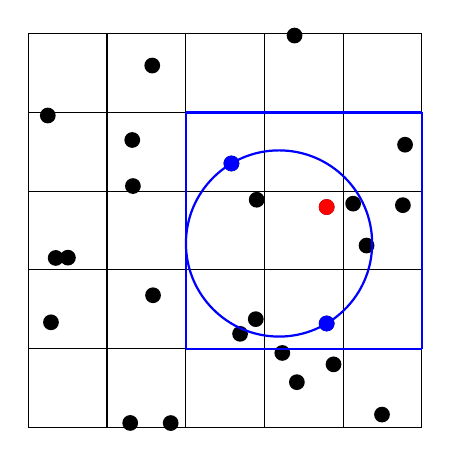
\begin{tikzpicture}
    \foreach \x in {0,1,...,5}{
        \draw (0,\x) -- (5,\x);
        \draw (\x,0) -- (\x,5);
    }
    %random numbers generated by Python
    \foreach \x / \y in {0.28897762565/1.33479488842, 1.29507843519/0.0567389232558, 1.32094528703/3.65045643132, 2.90131976409/2.89143039453, 3.38227004393/4.97678250754, 4.78587153595/3.59043085053, 4.49289684902/0.16312339617, 2.88976245038/1.37508072608, 0.503908610931/2.15612491084, 4.29648323686/2.30979809325, 1.57506933975/4.5958939884, 3.41193951077/0.574638720997, 1.58494426782/1.67834825887, 3.87742721851/0.800878920581, 0.34861369265/2.15217676901, 3.78999774171/1.31996000053, 3.22671310651/0.945568165194, 2.58060642147/3.3521091272, 1.8091306587/0.055518765505, 4.12621981945/2.84187520295, 2.69064049175/1.18843544815, 0.248568008024/3.96126629448, 1.32959523341/3.0654517407, 4.7582022563/2.8223407318, 3.78979061396/2.79890572216}{
        \fill (\x, \y) circle(0.1);
    }
    %~ 2.58060642147/3.3521091272
    %~ 3.78999774171/1.31996000053
    \def\xa{2.58060642147}
    \def\ya{3.3521091272}
    \def\xb{3.78999774171}
    \def\yb{1.31996000053}
    \def\x{3.1853020815900002}
    \def\y{2.3360345638649997}
    \def\d{1.1823977163477497}
    \fill[blue] (\xa,\ya) circle(0.1);
    \fill[blue] (\xb,\yb) circle(0.1);
    \fill[red] (3.78979061396,2.79890572216) circle(0.1);
    \draw[blue,thick] (2,1) -- (5,1);
    \draw[blue,thick] (2,4) -- (5,4);
    \draw[blue,thick] (2,1) -- (2,4);
    \draw[blue,thick] (5,1) -- (5,4);
    \draw[blue,thick] (\x, \y) circle(\d);
\end{tikzpicture}

            }
            \subfigure[Connected Nodes][]{
                \label{sfig:cell:small}
                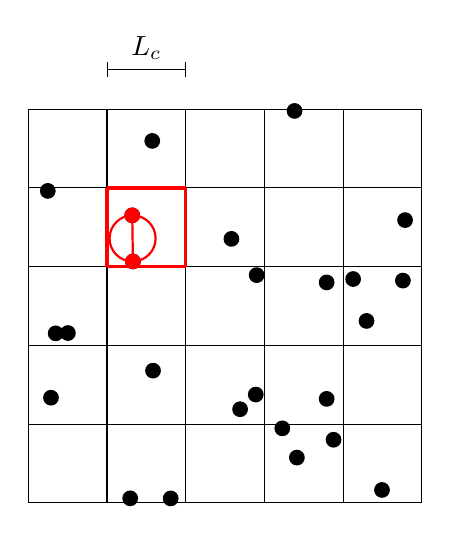
\begin{tikzpicture}
    \draw[|-|] (1,5.5) -- node[above] {$L_c$} (2,5.5);
    \foreach \x in {0,1,...,5}{
        \draw (0,\x) -- (5,\x);
        \draw (\x,0) -- (\x,5);
    }
    %random numbers generated by Python
    \foreach \x / \y in {0.28897762565/1.33479488842, 1.29507843519/0.0567389232558, 1.32094528703/3.65045643132, 2.90131976409/2.89143039453, 3.38227004393/4.97678250754, 4.78587153595/3.59043085053, 4.49289684902/0.16312339617, 2.88976245038/1.37508072608, 0.503908610931/2.15612491084, 4.29648323686/2.30979809325, 1.57506933975/4.5958939884, 3.41193951077/0.574638720997, 1.58494426782/1.67834825887, 3.87742721851/0.800878920581, 0.34861369265/2.15217676901, 3.78999774171/1.31996000053, 3.22671310651/0.945568165194, 2.58060642147/3.3521091272, 1.8091306587/0.055518765505, 4.12621981945/2.84187520295, 2.69064049175/1.18843544815, 0.248568008024/3.96126629448, 1.32959523341/3.0654517407, 4.7582022563/2.8223407318, 3.78979061396/2.79890572216}{
        \fill (\x, \y) circle(0.1);
    }
    %~ 1.32094528703/3.65045643132
    %~ 1.32959523341/3.0654517407
    \def\xa{1.32094528703}
    \def\ya{3.65045643132}
    \def\xb{1.32959523341}
    \def\yb{3.0654517407}
    \def\x{1.3252702602199999}
    \def\y{3.3579540860099999}
    \def\d{0.29253431833708793}
    \fill[red] (\xa,\ya) circle(0.1);
    \fill[red] (\xb,\yb) circle(0.1);
    \draw[red,very thick] (1,3) -- (2,3);
    \draw[red,very thick] (1,4) -- (2,4);
    \draw[red,very thick] (1,3) -- (1,4);
    \draw[red,very thick] (2,3) -- (2,4);
    \draw[red,thick] (\x, \y) circle(\d);
    \draw[red,thick] (\xa, \ya) -- (\xb, \yb) ;
\end{tikzpicture}

            }
            \caption[Sketch how the Cell Method works]
            {
                Sketch how the cell algorithm for the construction of the
                RNG and GG works. Here with the lune definition of the GG.
                The bounding box of the lune which determines which cells have
                to be tested, is marked with thick colored lines.
                \subref{sfig:cell:big} shows that it is sufficient to find a
                single node in an inner cell of the bounding box to discard
                the edge between two distant nodes. The nodes inside the
                other 8 marked cells do not have to be tested anymore.
                \subref{sfig:cell:small} shows that only the nodes inside the
                marked cell have to be tested, because there are no other nodes,
                the edge can be drawn.
            }
            \label{fig:cell}
        \end{figure}\\
        Given the discretized cell structure it is just necessary to test the nodes in the cells which
        resemble a rectangular bounding box of the lune. Most pairs will be
        far away from each other and there will be one or more cells in the
        middle of the bounding box, which are completely inside the lune so.
        Then only one node has to be tested from such a cell to discard an
        edge between the nodes. On the other hand, nodes that will be connected
        are near to each other so that only very few cells intersect the bounding
        box of their lune and consequently only very few nodes have to be tested.\\
        Here the number of cells equals the number of nodes.
        Indeed this method reduced the time needed to construct a RNG with
        \(N=32^2\) and \(N=64^2\) by a factor of
        over \(15\) respectively \(40\). Though the complexity is still of
        order \(O(N^2)\) in the best case, because for every pair at least
        one check has to be performed.
